\documentclass[UTF8]{ctexart}
\usepackage{xcolor}
\usepackage{amsmath}
\usepackage{bm}
\usepackage{amssymb}
\usepackage[colorlinks,linkcolor=blue,citecolor=black]{hyperref}
\usepackage{graphicx}
\usepackage{subfigure}
\usepackage{caption}
\usepackage{tocbibind}
\usepackage{geometry}
\geometry{bottom=3cm}

\usepackage{tikz}
\usetikzlibrary{quotes,angles}

\begin{document}

\section{第一次记录}
\subsection{问题描述}
已知目标和平台在平面 $XOY$ 上运动,$XOY$ 坐标系的刻度单位为千米。

\begin{figure}[h]
    \centering
    \includegraphics[scale=0.8]{fig1.jpg}
    \caption{目标与平台示意图}
\end{figure}
平台沿 $X$ 轴正向运动,起始位置为 $(10,0)$,终止位置为 $(13,0)$。平台的运动速度为 0.05km/s,因此运动总时间为60s。
目标沿任意曲线运动。平台与目标连线和 $X$ 轴正向的夹角为 $\theta$。

\subsection{建立模型}
\subsubsection{任意曲线}
假设目标在平面内沿任意曲线运动,在仅有角度测量值 $\theta$ 的情况下,如图\ref{fig:1}所示。显然,在未知目标速度,运动规律的情况下,任意经过
射线 $l_1,l_2,l_3$ 的曲线都可做为该区域目标的移动曲线,即解不唯一。

\begin{figure}[h]
    \centering
    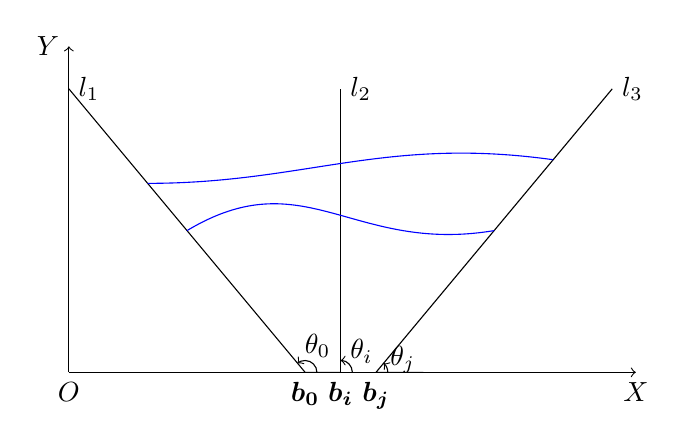
\begin{tikzpicture}[scale=0.6]
        \draw[->] (0,0) -- (12,0);
        \draw[->] (0,0) -- (0,6.9);
        \draw (0,0) node[below] {$O$};
        \draw (12,0) node[below] {$X$};
        \draw (0,6.9) node[left] {$Y$};
        \coordinate (b) at (5,0);
        \coordinate (c) at (5.75,0);
        \coordinate (x) at (0,6);
        \coordinate (d) at (5.75,6);
        \coordinate (e) at (7.5,0);
        \coordinate (f) at (6.5,0);
        \coordinate (g) at (11.5,6);
        \draw (x) node[right] {$l_1$} -- (b) node[below] {$\bm{b_0}$} -- (c) node[below] {$\bm{b_i}$ } 
        pic [draw, ->, "$\theta_0$", angle radius=1.5mm, angle eccentricity=2.5] {angle = c--b--x};
        \draw (e) -- (c) -- (d) node[right] {$l_2$}
        pic [draw,->,"$\theta_i$", angle radius=1.5mm, angle eccentricity=2.5 ] {angle = e--c--d};
        \draw (e) -- (f) node[below] {$\bm{b_j}$} -- (g) node[right] {$l_3$}
        pic [draw, ->, "$\theta_j$", angle radius=1.5mm, angle eccentricity=2.5] {angle = e--f--g}; 

        \draw[blue] (2.5,3) .. controls (5,4.5) and (6,2.5) .. (9,3);
        \draw[blue] (5/3,4) .. controls (5,4) and (20/3,5) .. (10.25,4.5);

    \end{tikzpicture}
    \caption{沿任意曲线运动}\label{fig:1}
\end{figure}

\subsubsection{匀速直线运动}
\begin{enumerate}
    \item[A.] 目标速度未知
\end{enumerate} 

假设目标沿 $X$ 轴正向做匀速直线运动,速度未知记为 $v$。由于平台以速度 $v_b = 0.05$km/s,我们可将目标视为静止,平台沿 $X$ 轴负方向以速度 $v'_b = v-v_b$ 做匀速直线运动。如图\ref{fig:2}所示。

假设目标的初始位置坐标为 $\bm{x}=(x_T,y_T)^T$,每0.1s平台对应的位置分别为 $\bm{b_i}=(b_{ix},b_{iy})^T, i \in \lbrace 0,1,\cdots,600 \rbrace$,
其中 $\bm{b_0} = (10,0)^T$。每0.1s平台所测得目标与平台连线和 $X$ 轴正向的夹角为 $\theta_i,i \in \lbrace 0,1,2,\cdots,600 \rbrace$,$\theta_i$ 可测量。将 $\bm{x_i}$ 向 $X$ 轴负方向移动,使之与 $\bm{x}$ 重合。同时将 $\bm{b_i}$
保持对 $\bm{x_i}$ 位置不变进行相对移动,记移动后的点为 $\bm{b'_i}$。此时我们得到
\begin{equation}
    b'_{ix} = b_{0x} -0.1(i-0) v'_b \label{eq:1}
\end{equation}
根据几何关系我们得到
\begin{equation}
    \begin{cases}
        \frac{\|\bm{b'_i} - \bm{b_0} \|}{\sin (\theta_0 - \theta_i)} = \frac{\| \bm{x}-\bm{b_0} \| }{\sin \theta_i}\\
        x_T = b_{0x} + \| \bm{x} - \bm{b_0} \| \cos \theta_0 \\
        y_T = b_{0y} + \| \bm{x} - \bm{b_0} \| \sin \theta_0
    \end{cases}
\end{equation}
进而得到
\begin{equation}
    \begin{cases}
        x_T = b_{0x} + \frac{\| \bm{b'_i} - \bm{b_0} \| \sin \theta_i \cos \theta_0}{\sin (\theta_0 - \theta_i)} \\ 
        y_T = b_{0y} + \frac{\| \bm{b'_i} - \bm{b_0} \| \sin \theta_i \sin \theta_0}{\sin (\theta_0 - \theta_i)}
    \end{cases}
\end{equation}
将(\ref{eq:1})代入上式得
\begin{equation}
    \begin{cases}
        x_T = b_{0x} + \frac{0.1 (i-0)v'_b \sin \theta_i \cos \theta_0}{\sin (\theta_0 - \theta_i)} \\ 
        y_T = b_{0y} + \frac{0.1 (i-0)v'_b \sin \theta_i \sin \theta_0}{\sin (\theta_0 - \theta_i)}
    \end{cases}
\end{equation}
由上式可知,由于平台位置 $\bm{b_0}$ 已知,目标得初始位置 $\bm{x}$ 只与测量得方位角 $\theta_i$ 和 速度有关。在方位角 $\theta_i$ 已知得情况下,目标的初始位置 $\bm{x}$ 只与 目标的速度有关。


\begin{figure}[h]
\centering
\begin{tikzpicture}[scale=0.78]
    \draw[->] (0,0) -- (4.8,0);
    \draw[->] (0,0) -- (0,4.6);
    \draw (0,0) node[below] {$O$};
    \draw (4.8,0) node[below] {$X$};
    \draw (0,4.6) node[left] {$Y$};
    \coordinate (b) at (2,0);
    \coordinate (c) at (2.4,0);
    \coordinate (x) at (0,4);
    \coordinate (d) at (3.2,4);
    \coordinate (e) at (3,0);
    \draw (x) node[left] {$\bm{x}$} -- (b) node[below] {$\bm{b_0}$} -- (c) node[below] {$\bm{b_i}$ } 
    pic [draw, ->, "$\theta_0$", angle radius=1.5mm, angle eccentricity=2.5] {angle = c--b--x};
    \draw (e) -- (c) -- (d) node[right] {$\bm{x_i}$}
    pic [draw,->,"$\theta_i$", angle radius=1.5mm, angle eccentricity=2.5 ] {angle = e--c--d};
    \draw (x)--(d);
    
    \draw[->] (5,2.3) -- (8,2.3);
    \draw (6.5,2.5) node {将目标看做静止};
    
    \draw[->] (8,0) -- (14,0) node[below] {$X$};
    \draw[->] (11,0) -- (11,4.6) node[left] {$Y$};
    \draw (11,0) node[below] {$O$};
    \coordinate (f) at (13,0);
    \coordinate (g) at (10.2,0);
    \coordinate (h) at (11,4);
    \coordinate (j) at (13.5 ,0);
    \draw (j) -- (f) node[below] {$\bm{b_0}$} -- (h) node[left] {$\bm{x}(\bm{x_i})$}
    pic [draw, ->, "$\theta_0$", angle radius=1.5mm, angle eccentricity=2.5] {angle = j--f--h};
    \draw (f) -- (g) node[below] {$\bm{b'_i}$} -- (h)
    pic [draw, ->, "$\theta_i$", angle radius=1.5mm, angle eccentricity=2.5] {angle = f--g--h}; 
\end{tikzpicture}
\caption{平台相对于静止的目标的位置变换}\label{fig:2}
\end{figure}
\begin{enumerate}
    \item[B.] 速度已知 
\end{enumerate}

假设目标沿 $X$ 轴正向做匀速直线运动,速度 $v=0.38$km/s。则可以看做目标位置不动,平台沿 $X$ 轴负方向以速度 $v'=0.33$km/s 做匀速直线运动。同样如图\ref{fig:2}所示,关于各点的坐标我们做与 A 相同的假设。即目标的初始位置
为 $\bm{x}$ 未知,平台的坐标为 $\bm{b_i}$ 已知,进行变换后对应的位置为 $\bm{b'_i}$,方位角$\theta_i$已知。根据位置关系我们得到
\begin{equation}
    b'_{ix} = b_{0x} - 0.1(i-0)v'
\end{equation}
根据几何关系可得到
\begin{equation}
    \theta_i = \arctan \frac{y_T-b'_{iy}}{x_T-b'_{ix}}
\end{equation}
由于测量的角度存在噪声,假设每次测量的噪声变量互相独立,且满足高斯分布,即噪声变量 $\eta_i \sim N(0,\sigma^2)$,则测量值 $\tilde{\theta_i}$ 满足
\begin{equation}
    \tilde{\theta_i} = \arctan \frac{y_T-b'_{iy}}{x_T-b'_{ix}} + \eta_i, \quad i \in \lbrace 0,1,\cdots,600 \rbrace
\end{equation}
记 $\bm{\theta} = [\theta_0, \theta_1, \cdots, \theta_{600}]$。然后得到
\begin{equation}
    P(\bm{\theta} | \bm{x}) = \prod\limits_{i = 0}^{600} {\frac{1}{{\sqrt {2\pi } \sigma }}\exp \{  - \frac{{\eta _i^2}}{{2{\sigma ^2}}}\} } 
\end{equation}
利用最大似然算法 (ML) 求解[1]目标的初始坐标 $(x_T, y_T)$应得
\begin{equation}
    \begin{split}
        \hat{\bm{x}} =& \mathop {\arg \min }\limits_{({x_T},{y_T})} \frac{\sum\limits_{i=0}^{600} \eta_i^2}{2 \sigma^2} \\
                    =& \mathop {\arg \min}\limits_{(x_T,y_T)} \frac{\sum\limits_{i=0}^{600} (\hat{\theta_i}-\arctan\frac{y_T-b'_{iy}}{x_T-b'_{ix}})^2}{2\sigma^2}
    \end{split}
\end{equation}
这个问题求解很困难,并且可能存在多个解[1],因此我们考虑最小二乘法 (LS)\\
当噪声变量足够小时,即 $\eta_i \approx 0$,得到
\begin{equation}
    \tilde{\theta_i} \approx \arctan \frac{y_T-b'_{iy}}{x_T-b'_{ix}} , \quad i \in \lbrace 0,1,\cdots,600 \rbrace
\end{equation}
变换得到
\begin{equation}
    \tan \tilde{\theta_i} \approx \frac{y_T-b'_{iy}}{x_T-b'_{ix}} \implies (y_T-b'_{iy})\cos \tilde{\theta_i} - (x_T-b'_{ix})\sin \tilde{\theta_i} \approx 0
\end{equation}
利用 LS 算法[2],我们得到
\begin{equation}
    \hat{\bm{x}} = \mathop {\arg \min}\limits_{(x_T,y_T)} \sum\limits_{i=0}^{600} ((y_T-b'_{iy})\cos \tilde{\theta_i} - (x_T-b'_{ix})\sin \tilde{\theta_i})^2 \label{eq:2}
\end{equation}
令
\begin{equation*}
    \bm{A} = \begin{bmatrix}
        -\sin \tilde{\theta_0} & \cos \tilde{\theta_0} \\
        -\sin \tilde{\theta_1} & \cos \tilde{\theta_1} \\
        \vdots & \vdots \\
        -\sin \tilde{\theta_{600}} & \cos \tilde{\theta_{600}}
    \end{bmatrix}, \qquad 
    \bm{b} = \begin{bmatrix}
        -\sin \tilde{\theta_0} & \cos \tilde{\theta_0} \\
        -\sin \tilde{\theta_1} & \cos \tilde{\theta_1} \\
        \vdots & \vdots \\
        -\sin \tilde{\theta_{600}} & \cos \tilde{\theta_{600}}
    \end{bmatrix}\begin{bmatrix}
        b'_{ix} \\
        b'_{iy}
    \end{bmatrix}
\end{equation*}
(\ref{eq:2})可以描述为
\begin{equation}
    \hat{\bm{x}} = \mathop{\arg \min}\limits_{\bm{x}} \| \bm{A}\bm{x} -\bm{b} \|_2^2
\end{equation}
于是可解得
\begin{equation}
    \hat{\bm{x}} = (\bm{A}^T \bm{A})^{-1} \bm{A}^T \bm{b} 
\end{equation}

\subsection{测试数据}
根据已有数据利用上述方法,取 $\sigma = 10^{-4}$,得到 $\hat{\bm{x}}=(0.000095km,19.999528km)^T$,真实坐标 $\bm{x}=(0km,20km)^T$

\begin{figure}[h]
    \centering
    \subfigure[估计位置vs真实位置]{
        \includegraphics[scale=0.34]{fig3.png}
    }
    \subfigure[相对于平台位置]{
        \includegraphics[scale=0.35]{fig4.png}
    }
\end{figure}

\section{RSS-AOA}
\subsection{RSS测量值转换}
根据[2]中所述,有
\begin{equation}
    L_{ij} = 10\log_{10} (P_T/P_{ij}) (dB)
\end{equation}
其中,$L_{ij}$ 表示第 $i$ 个传感器与第 $j$ 个传感器之间的路径损失(path loss),$P_T$ 代表
传感器的传输功率 (transmission power),$P_{ij}$ 代表接收功率 (received power),$L_{ij}$ 的单位为 dB。
\begin{equation}
    L_{ij} = L_0 + 10 \gamma \log_{10} \frac{\| \bm{x_i}-\bm{x_j} \| }{d_0}
\end{equation}
其中,$L_0$ 表示在参考距离 $d_0$ 处的路径损失值 $(\| \bm{x_i}- \bm{x_j} \| \geq d_0)$,$\gamma$ 是路径损失系数,
表示随距离增加路径损失的变化率
\begin{figure}
    \centering
    \includegraphics[scale=0.5]{fig2.png}
    \caption{轨迹2运动图像}
\end{figure}

\small
\begin{thebibliography}{00}
    \bibitem{b1} Yichao Cao, "Target Localization Based on Angle of Arrivals",\emph{Journal of Electronic Science and Technology of China},2007, vol. 5, no. 2, 172-174
    \bibitem{b2} Tomic S,Beko M and Dinis R,"3-D Target Localization in Wireless Sensor Networks Using RSS and AoA Measurements",
    \emph{IEEE Transactions on Vehicular Technology}, 2016, 66(4):3197-3210
    \bibitem{b3} Tomic S, Beko M and Dinis R, et al, "On Target Localization Using Combined RSS and AoA Measurements", \emph{Sensors}, 2018, 12(4):1266
    \bibitem{b4} Tomic S, Beko M and Dinis R, et al, "Distributed algorithm for target localization in wireless sensor networks using RSS and AoA measurements",
    \emph{Pervasive and Mobile Computing}, 2017, 37:63-77
    \bibitem{b5} Tomic S,Beko M and Tuba M,"A Linear Estimator for Network Localization Using Integrated RSS and AOA Measurements",
    \emph{IEEE Signal Processing Letters}, 2019, 26(3):405-409

\end{thebibliography}

\end{document}